\documentclass[11pt,a4paper,fontset=fandol]{ctexart}

% ══════════════════════════════════════════════════════════════
% Packages
% ══════════════════════════════════════════════════════════════
\usepackage[margin=1in]{geometry}
\usepackage{amsmath,amssymb}
\usepackage{graphicx}
\usepackage{booktabs}
\usepackage{xcolor}
\usepackage{hyperref}
\usepackage{caption}
\usepackage{enumitem}
\usepackage{tabularx}
\usepackage{float}
\usepackage{fancyvrb}

\graphicspath{{../figures/}}

\setlength{\emergencystretch}{3em}
\hyphenpenalty=1500
\exhyphenpenalty=100

\hypersetup{
  colorlinks=true,
  linkcolor=blue!70!black,
  citecolor=green!50!black,
  urlcolor=blue!60!black,
}

\captionsetup{font=small,labelfont=bf}

\newcommand{\code}[1]{\texttt{#1}}

% ══════════════════════════════════════════════════════════════
% Title
% ══════════════════════════════════════════════════════════════
\title{\textbf{Fugue}：通过嫁接冻结生成器\\实现乐谱条件音乐改编}
\author{Jing Zhang\thanks{代码、示例与评估记录：\url{https://github.com/HenryZ838978/fugue}}\\[0.3em]\normalsize 独立研究}
\date{2026 年 9 月}

\begin{document}

\maketitle

% ══════════════════════════════════════════════════════════════
\begin{abstract}
\noindent
实用的音乐改编（cover）既要让人仍能辨认出原曲，又要呈现不同的编曲和制作风格。Fugue 将 YuE2-3B 基于乐谱条件的生成能力与 MiniMax-Music3 基于扩散的声学渲染器相结合，无需更新任何一个预训练模型。一个拥有 66.6M 参数的适配器将 YuE2 的声学潜表示映射到渲染器现有的条件接口。该适配器不需要额外的原曲/改编曲配对数据或人工标注：其输入和目标均由 MM3 自身生成结果的音频及已保存的编码构建而来。在将 209 首真实歌曲各改编为两种目标风格的实验中，当前版本 Fugue v4 的原曲检索平均倒数排名（MRR）为 0.609，YuE2 原生解码器为 0.646，而仅使用风格条件的对照组为 0.022。对同一批 418 个生成潜表示进行解码时，频谱滚降频率的中位数从 13.8 kHz 提高至 17.6 kHz，立体声侧声道/中声道功率比从 $-10.9$ dB 提高至 $-4.8$ dB。这些测量描述的是 MM3 预训练 DiT 渲染路径带来的更多高频成分和更宽立体声声场，而非总体音质排名。我们发布了适配器、推理包、常驻服务、改编前端、评估记录和绘图代码。Fugue 将学习得到的跨模型接口与端到端部署、评估基础设施相结合，为乐谱条件音乐改编提供了一种实用的替代方案。
\end{abstract}

% ══════════════════════════════════════════════════════════════
\section{引言}
% ══════════════════════════════════════════════════════════════

音乐改编生成的起点，是用户已经希望保留的音乐素材。任务在于改变其呈现方式：例如，将一段人声录音改编为钢琴曲，或将同一首歌演绎为以吉他为主导的摇滚乐。因此，原曲身份保留、风格控制与声学渲染同样重要。即便输出在所要求的曲风中听起来颇具说服力，只要它丢失了预期的原曲身份，就不能算作成功的改编。

YuE2-3B~\cite{yue2} 提供乐谱条件音乐生成能力，支持 ABC 输入，并包含一个非自回归声学生成阶段。MiniMax-Music3（MM3）~\cite{mm3} 提供 Fugue 声学渲染所使用的预训练扩散 Transformer 和立体声声码器。我们使用前者生成受乐谱控制的音乐内容，使用后者进行渲染。两个模型通过学习得到的潜表示映射，在波形解码之前连接起来。最终系统为音乐改编提供了另一条路径：在配对评估中，相比原生解码器，它呈现出更多高频成分和更宽立体声声场。

\begin{figure}[t]
    \centering
    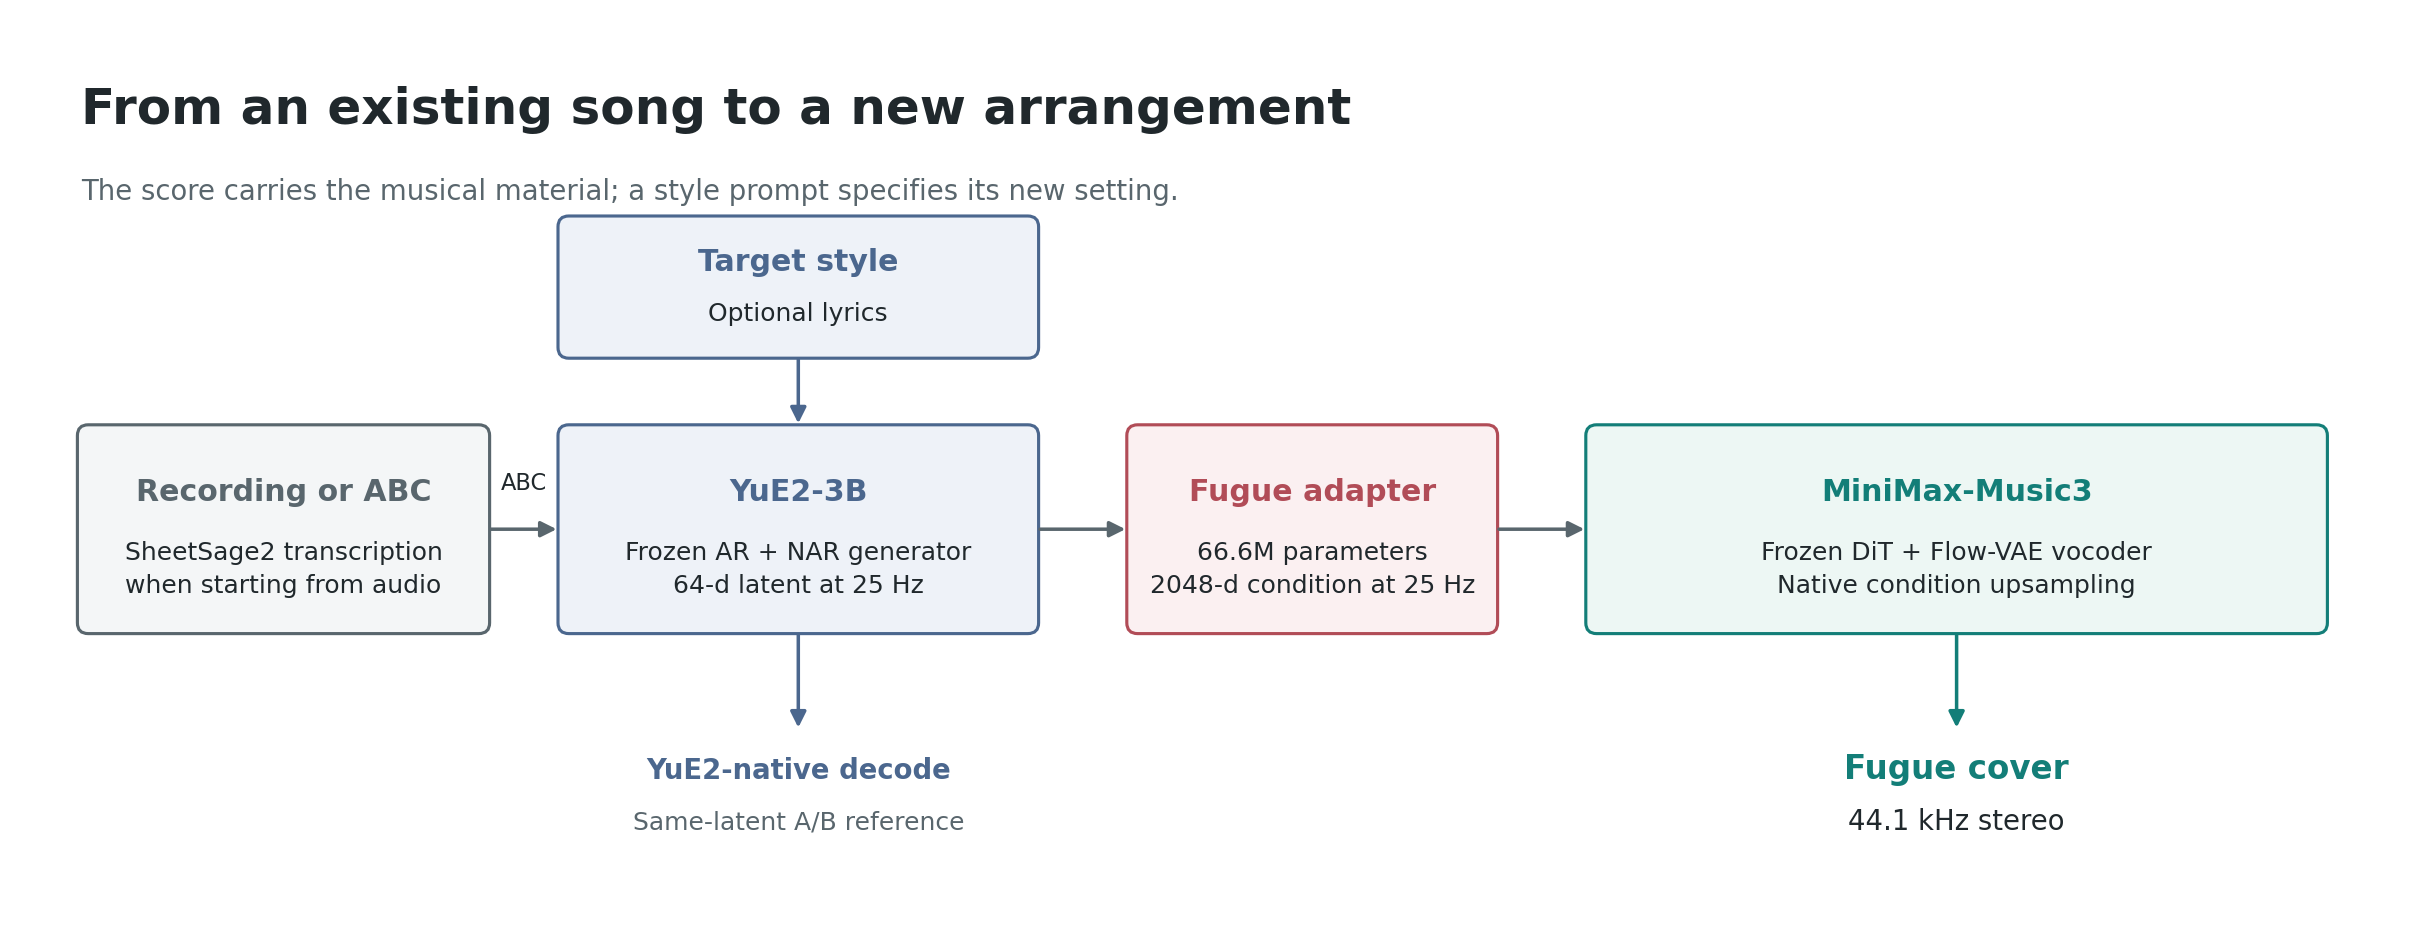
\includegraphics[width=0.96\linewidth]{cover-workflow.png}
    \caption{Fugue 推理流程及其原生解码器参考分支。将录音转录为 ABC，或直接提供乐谱。YuE2 在乐谱与风格提示词的条件下生成声学潜表示。Fugue 将该潜表示映射为 MM3 原生的 DiT 条件。YuE2 原生解码器提供配对参考，用于单独考察渲染环节的变化。}
    \label{fig:workflow}
\end{figure}

\textbf{Fugue}（赋格）这一名称源于可辨识的主题在相互交织的音乐声部中反复回归。它表达了一项设计目标：在人声或器乐旋律线中保持连续性，同时允许其周围的音乐环境发生变化并作出呼应。当前系统通过受乐谱条件控制的混合音频生成来实现这一目标。

本研究的核心贡献是\textbf{一种无需额外原曲/改编曲配对监督即可组合既有能力的方法}。训练样本由保存了 RVQ 编码的 MM3 生成结果构建而来；无需将任何录音与人工或模型制作的改编版本配对。我们还确定了一个可用的跨模型接口，校正了分块渲染引入的时间轴错位，并在真实歌曲改编任务上评估了最终系统。主要实验见第~\ref{sec:eval}~节；直接在 MM3 中训练乐谱条件控制能力的失败尝试保留在附录~\ref{app:direct}~中。

第二项贡献是\textbf{让这一组合可用、可检查的基础设施}：训练样本对提取流水线、包含归一化统计量的适配器封装、可在同一张 GPU 上运行的独立常驻服务、改编 CLI 与前端、长音频分块推理，以及可续跑的配对评估。第~\ref{sec:infra}~节介绍这些组件，并区分 Fugue 的集成工作与冻结模型原有的能力。

% ══════════════════════════════════════════════════════════════
\section{方法}
% ══════════════════════════════════════════════════════════════

\subsection{训练与推理共用的接口}

YuE2 的自回归（AR）路径生成语义 token，非自回归（NAR）流匹配阶段则生成维度为 64、帧率为 25 Hz 的声学潜表示 \code{z}。公开的 YuE2 VAE 编码器也将音频映射为相同格式的潜表示。我们选择这一表示，是因为训练音频与乐谱条件生成过程都能提供它。YuE2 的 NAR 隐藏状态会随去噪步骤变化，并非此处采用的固定接口。

MM3 通常根据其语言模型和 RVQ 深度解码器的隐藏状态构建 DiT 条件。我们将 \code{ConditionEncoder} \textbf{时间上采样之前}的 2048 维输出作为目标，记为 \code{c25}。适配器根据 \code{z} 预测 \code{c25}；随后，MM3 的上采样模块、DiT 和声码器保持不变地运行。主要的改编生成路径不使用 YuE2 原生 VAE 解码器，也不使用 MM3 的语言模型（LM）及深度解码器。

\begin{Verbatim}[frame=single,fontsize=\small,samepage=true,xleftmargin=1em,xrightmargin=1em]
z: (T, 64), 25 Hz
    -> Fugue 适配器
    -> c25: (T, 2048), 25 Hz
    -> MM3 原生最近邻上采样
    -> 冻结的 DiT 和 Flow-VAE 声码器
    -> 44.1 kHz 立体声
\end{Verbatim}

两种表示的标称帧率相同。然而，MM3 的分块渲染会引入时间轴漂移，在构建配对训练数据时必须予以校正。

\subsection{来自自生成录音的监督}

配对语料包含 12,837 个 MM3 生成样本，总时长约 191 小时，每个样本均包含音频、RVQ 编码、描述文本和歌词。对于每个生成样本，我们构建：

\begin{enumerate}[leftmargin=2em,itemsep=0.2em]
    \item \textbf{输入：}将渲染后的音频从 44.1 kHz 重采样至 48 kHz，再用冻结的 YuE2 VAE 编码器进行编码。
    \item \textbf{目标：}将已保存的编码和原始提示词输入冻结的 MM3 语言模型与深度解码器，以教师强制（teacher forcing）方式运行，然后执行 \code{ConditionEncoder} 直至其投影层，恢复 \code{c25}。
\end{enumerate}

\begin{figure}[t]
    \centering
    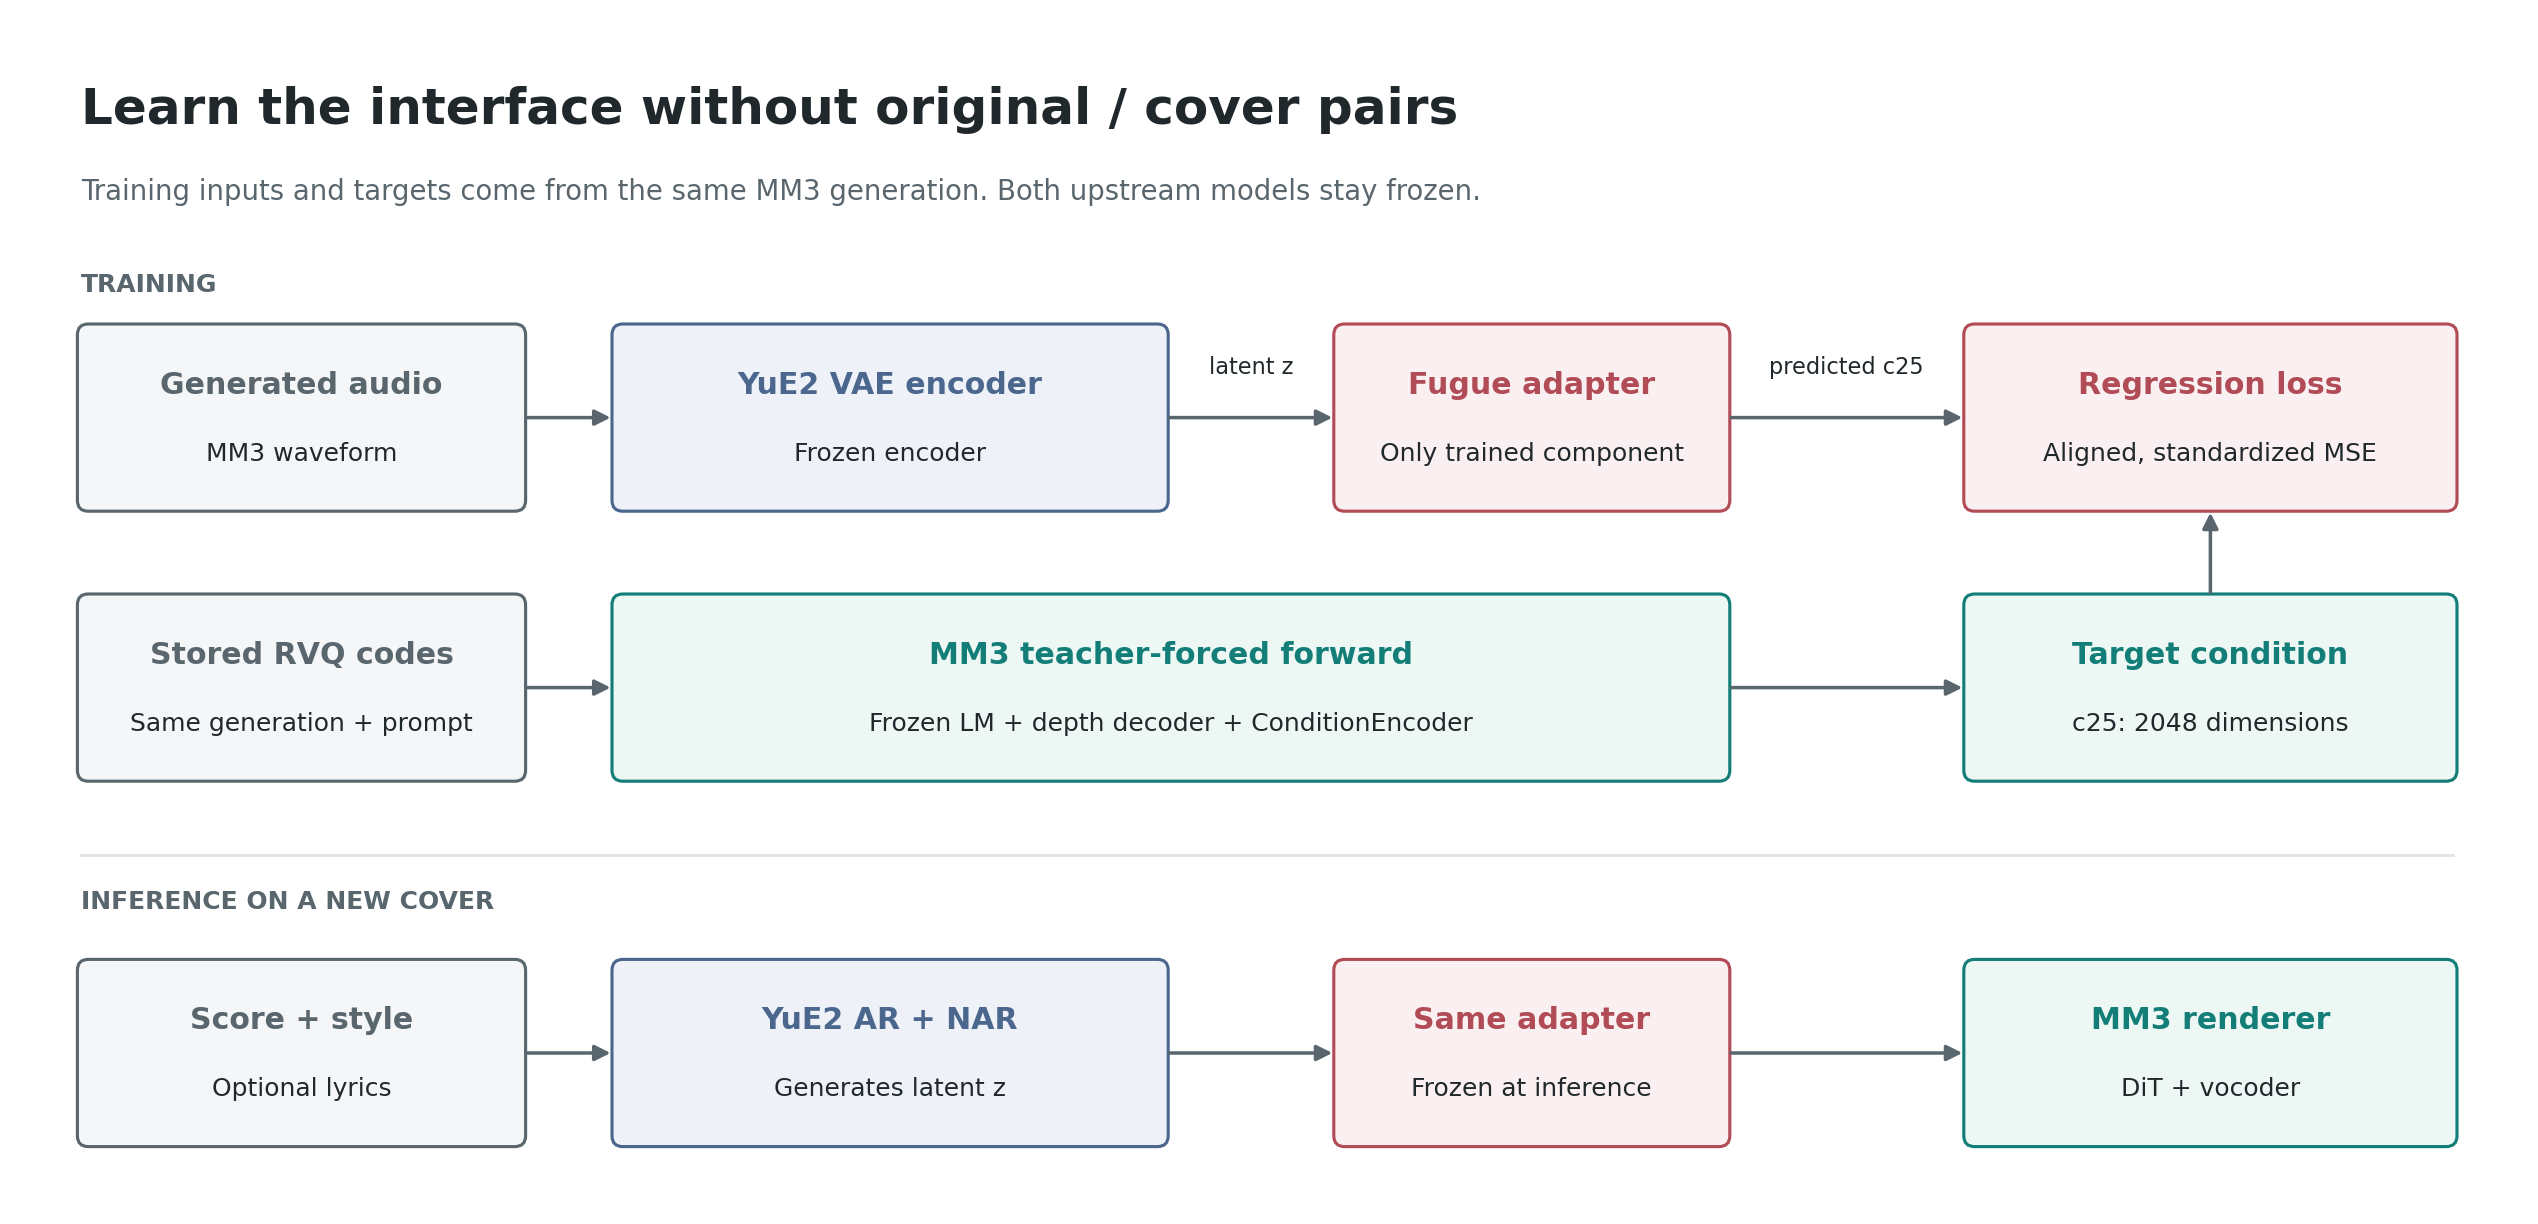
\includegraphics[width=0.96\linewidth]{training-pairs.png}
    \caption{训练与推理路径，突出展示共用适配器，以及如何从单个 MM3 生成样本中构建监督信号。一个训练样本对的两端描述的是同一段生成录音。推理时，YuE2 的乐谱条件 AR/NAR 生成器替代 VAE 编码器，成为 \code{z} 的来源。只有适配器参与优化。此适配阶段不使用原曲/改编曲配对数据。}
    \label{fig:pairs}
\end{figure}

保存生成时的编码，使我们无需使用 MM3 尚未公开的音频到 RVQ 量化器。在一项重建检查中，用教师强制方式恢复的条件进行渲染，结果与已保存原始音频之间的 log-mel L1 距离为 0.686；作为比较，使用不同 DiT 随机种子的两次渲染之间，该距离为 0.698。这为条件恢复的一致性提供了实证检查。

训练使用编码器产生的潜表示，而改编推理使用 NAR 生成的潜表示。两者格式相同，但分布未必相同。因此，我们对各通道进行归一化，并向训练输入添加高斯噪声。真实歌曲改编评估检验了从转录、YuE2 生成到适配器的完整路径。

\paragraph{时间对齐。}MM3 使用长度为 200 帧、步长为 100 帧的窗口进行渲染。每个完整窗口生成 689 帧声学潜表示；拼接时，每个步长实际推进 345 帧潜表示，而非标称的 344.53125 帧。因此，MM3 条件的第 $j$ 帧大致对应 YuE2 的以下帧位置：

\begin{Verbatim}[frame=single,fontsize=\small,samepage=true,xleftmargin=1em,xrightmargin=1em]
m(j) = round(j + 0.136054 * k(j))
k(j) = 0                              if j < 125
       floor((j - 25) / 100)           otherwise
\end{Verbatim}

实现中将 $k(j)$ 的上界限制为最后一个渲染窗口，并将所得输入索引裁剪至有效范围。该系数为 $345 / (441/128) - 100$。在对齐实验中，校正这一漂移后，使用三帧上下文的岭回归探针的 $R^2$ 从 0.262 提高至 0.347。

\subsection{适配器与优化}

适配器由以下部分组成：一个从 64 维到 768 维的线性投影层，两个卷积核大小为 5 的局部残差卷积，一个卷积核大小为 63、分组数为 16 的分组位置残差卷积，八个采用前置层归一化（pre-LN）、含 12 个注意力头的双向 Transformer 层，以及最终的归一化层和从 768 维到 2048 维的投影层。模型共有 66.6M 参数，不使用绝对位置嵌入。

输入和目标均按通道进行标准化。设 \code{y\_tc} 为标准化后的目标，\code{a\_tc} 为适配器预测，\code{sigma\_c} 为原始目标通道的标准差。带掩码的损失为：

\begin{Verbatim}[frame=single,fontsize=\small,samepage=true,xleftmargin=1em,xrightmargin=1em]
w_c = 0.5 + 0.5 * sigma_c^2 / mean_c(sigma_c^2)
L   = mean_valid_frames [ mean_c (w_c * (a_tc - y_tc)^2) ]
\end{Verbatim}

输入噪声在标准化尺度下的标准差为 0.15。适配器使用 10,340 首歌曲训练，优化器为 AdamW，学习率为 3e-4，采用预热和余弦衰减，共训练 20,000 步，每个批次包含 24 个长度为 768 帧的裁剪片段。完成特征提取后，v4 训练在一张 RTX 4090 上耗时 67 分钟。语料生成和特征提取还需额外开销；实测对整个语料执行教师强制计算与 VAE 编码，分别约需 53 和 74 个单 GPU 分钟。

推理时，适配器使用 768 帧窗口进行预测，两侧各保留 128 帧上下文，避免对整首歌曲执行二次复杂度的注意力计算。在交给 MM3 渲染之前，对输出通道进行反标准化。YuE2 生成和声学渲染使用独立的随机种子。

% ══════════════════════════════════════════════════════════════
\section{真实歌曲改编评估}
\label{sec:eval}
% ══════════════════════════════════════════════════════════════

\subsection{评估方案}

本地基准沿用历史名称 \code{ood216}，包含来自日本/中国流行音乐及原声音乐曲库的 210 段录音，并配有 SheetSage2 转录结果。其中一份转录超出了 YuE2 的上下文长度限制，因此完整乐谱条件下保留了 \textbf{209 首原曲}。每首歌各生成两种目标风格，共得到 \textbf{418 个潜表示}，每个潜表示均分别由 YuE2 原生 VAE 和 Fugue v4 解码。检索库仍包含\textbf{全部 210 段原始录音}。

六种目标风格分别为钢琴抒情曲、英伦吉他摇滚、爵士三重奏、合成器浪潮（synthwave）、原声民谣和管弦乐电影配乐。按照 \code{eval\_gen.py} 的设定，每首歌分配到此列表中相隔三个位置的两种风格。生成结果均为纯器乐，仅生成前 60 秒，YuE2 随机种子为 0；Fugue 使用 DiT 随机种子 7，运行 30 步。无乐谱对照使用 \code{cot=off}，为每首歌采用其被分配的第一种风格，并使用两个解码器分别解码，每个解码器各得到 210 个输出。

原曲身份保留通过 Discogs-VINet~\cite{discogsvi} 的余弦相似度检索进行衡量，匹配的原始录音是检索库中唯一的相关项。风格通过 \code{laion/larger\_clap\_music\_and\_speech} 的 CLAP 音频/文本余弦相似度进行衡量。乐谱遵循程度则通过 SheetSage2 对输出重新转录，并对器乐声部的音程序列计算动态时间规整（DTW）来衡量。转录音符不足的输出不纳入 DTW 汇总统计。

这是一项本地配对渲染器评估，而非对完整 SHS100K 基准的复现。将每段原始录音的前 60 秒作为查询，在完整录音检索库中检索，可得到一组参考结果：Hit@1 为 0.819，Hit@10 为 0.933，MRR 为 0.861。

\subsection{同时考察原曲身份与风格}

\begin{figure}[t]
    \centering
    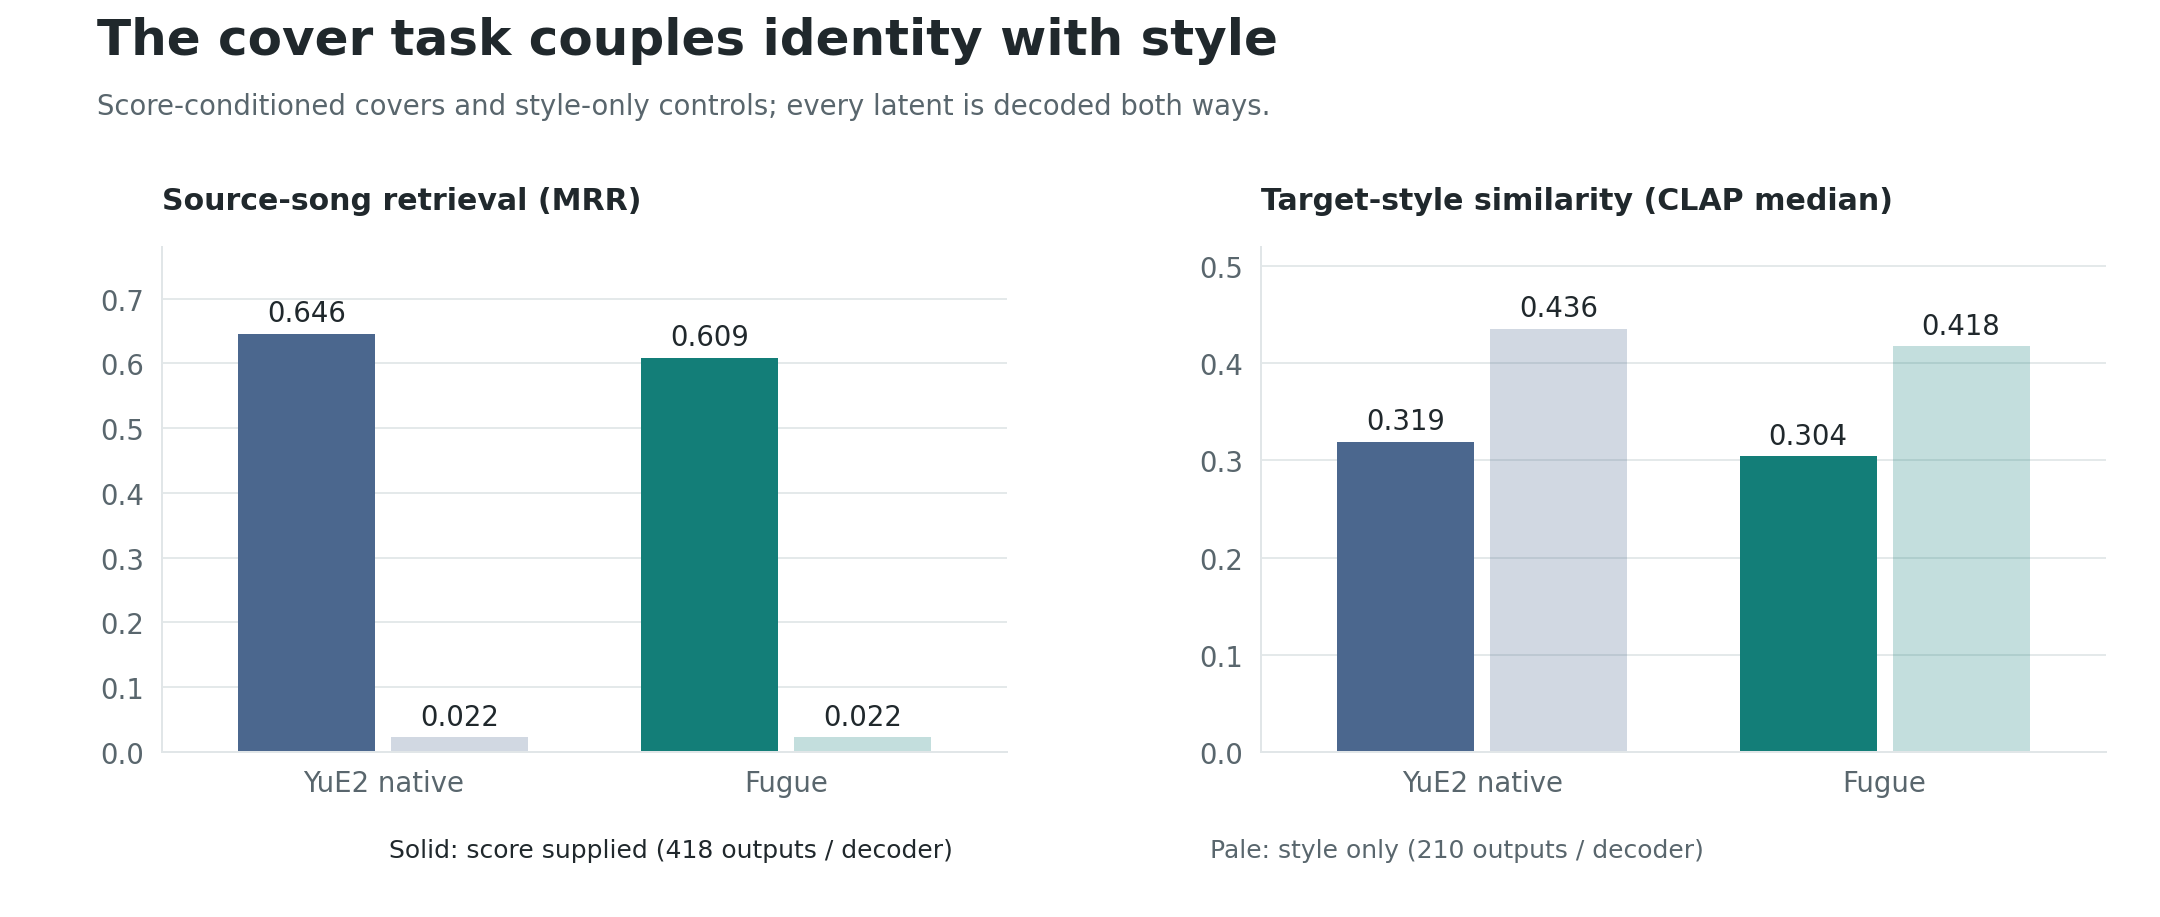
\includegraphics[width=0.96\linewidth]{identity-and-style.png}
    \caption{两个解码器在有、无原曲乐谱条件下的原曲身份与风格指标。原曲身份与目标风格衡量的是不同要求。移除乐谱后，整体 CLAP 中位数提高，但原曲检索性能降至接近随机水平。对照组每首歌使用一种风格；乐谱条件评估每首歌使用两种风格。}
    \label{fig:identity}
\end{figure}

\begin{table}[htbp]
    \centering
    \caption{本地改编基准上的原曲身份与风格指标。两种条件均使用 YuE2 生成，区别在于是否提供原曲乐谱。}
    \label{tab:identity}
    \small
    \begin{tabular}{lrrrrr}
        \toprule
        输入与解码器 & $n$ & Hit@1 & Hit@10 & MRR & CLAP 中位数 \\
        \midrule
        原曲乐谱，YuE2 原生解码器 & 418 & 0.557 & 0.809 & 0.646 & 0.319 \\
        \textbf{原曲乐谱，Fugue} & \textbf{418} & \textbf{0.524} & \textbf{0.775} & \textbf{0.609} & \textbf{0.304} \\
        仅风格，YuE2 原生解码器 & 210 & 0.000 & 0.033 & 0.022 & 0.436 \\
        仅风格，Fugue & 210 & 0.000 & 0.033 & 0.022 & 0.418 \\
        \bottomrule
    \end{tabular}
\end{table}

当前版本 Fugue v4 保留了原生解码器 94\% 的 MRR，其 Hit@1 低 3.35 个百分点。在共用潜表示的配对输出中，原曲检索排名在 239 对中保持不变，在 63 对中 Fugue 更优，在 116 对中 YuE2 原生解码器更优。配对 CLAP 差值的中位数为 $-0.019$。这些结果刻画的是当前适配器及渲染配置：系统保留了大部分原曲识别能力，同时仍存在可测量的检索差距。

这一差距可能与多种因素有关。适配器有限的回归精度可能改变歌曲特有的线索，而在 MM3 音频编码上训练，并不能消除与 YuE2 NAR 生成潜表示之间的分布差异。训练损失拟合的是 \code{c25}，而非直接优化原曲检索。渲染器引入的音色与空间呈现变化也可能改变检索嵌入。由于配对解码器接收相同的上游潜表示，这些解释针对的是适配器及渲染路径，而非不同的转录或生成输入。当前版本尚未单独确定各因素的贡献。

重新转录后的 DTW 中位数，YuE2 原生解码器为 0.470，Fugue 为 0.523，分别基于 372 和 375 个有效输出计算。在\textbf{两个解码器均有效的 372 对输出}中，配对差值的中位数为 0.000。相应的仅风格条件中位数为 1.686 和 1.622，两个解码器各有 197 个有效输出。

\subsection{高频成分与立体声声场}
\label{sec:acoustic}

此处测得的声学差异是更多高频能量和更宽立体声声场。这些渲染能力主要来自 MM3 预训练的 DiT 声学路径：DiT 合成声学潜表示，Flow-VAE 将其转换为立体声波形。Fugue 的贡献是提供一个接口，使 YuE2 生成的潜表示能够驱动这条路径，而无需重新训练其中任何一个组件。配对对比衡量的是适配器/DiT/声码器整条路径的综合效果，并未将 DiT 的贡献与声码器的贡献单独分离。

发布内容提供了相同潜表示下的 A/B 试听、两种风格的原曲与改编对比、一个人声示例，以及五个全长示例：一首器乐钢琴改编，以及两首基准集之外的真实录音各两种风格、共四首带人声的全长改编。这些示例用于展示和检查渲染差异，并非盲听评估。

\begin{figure}[t]
    \centering
    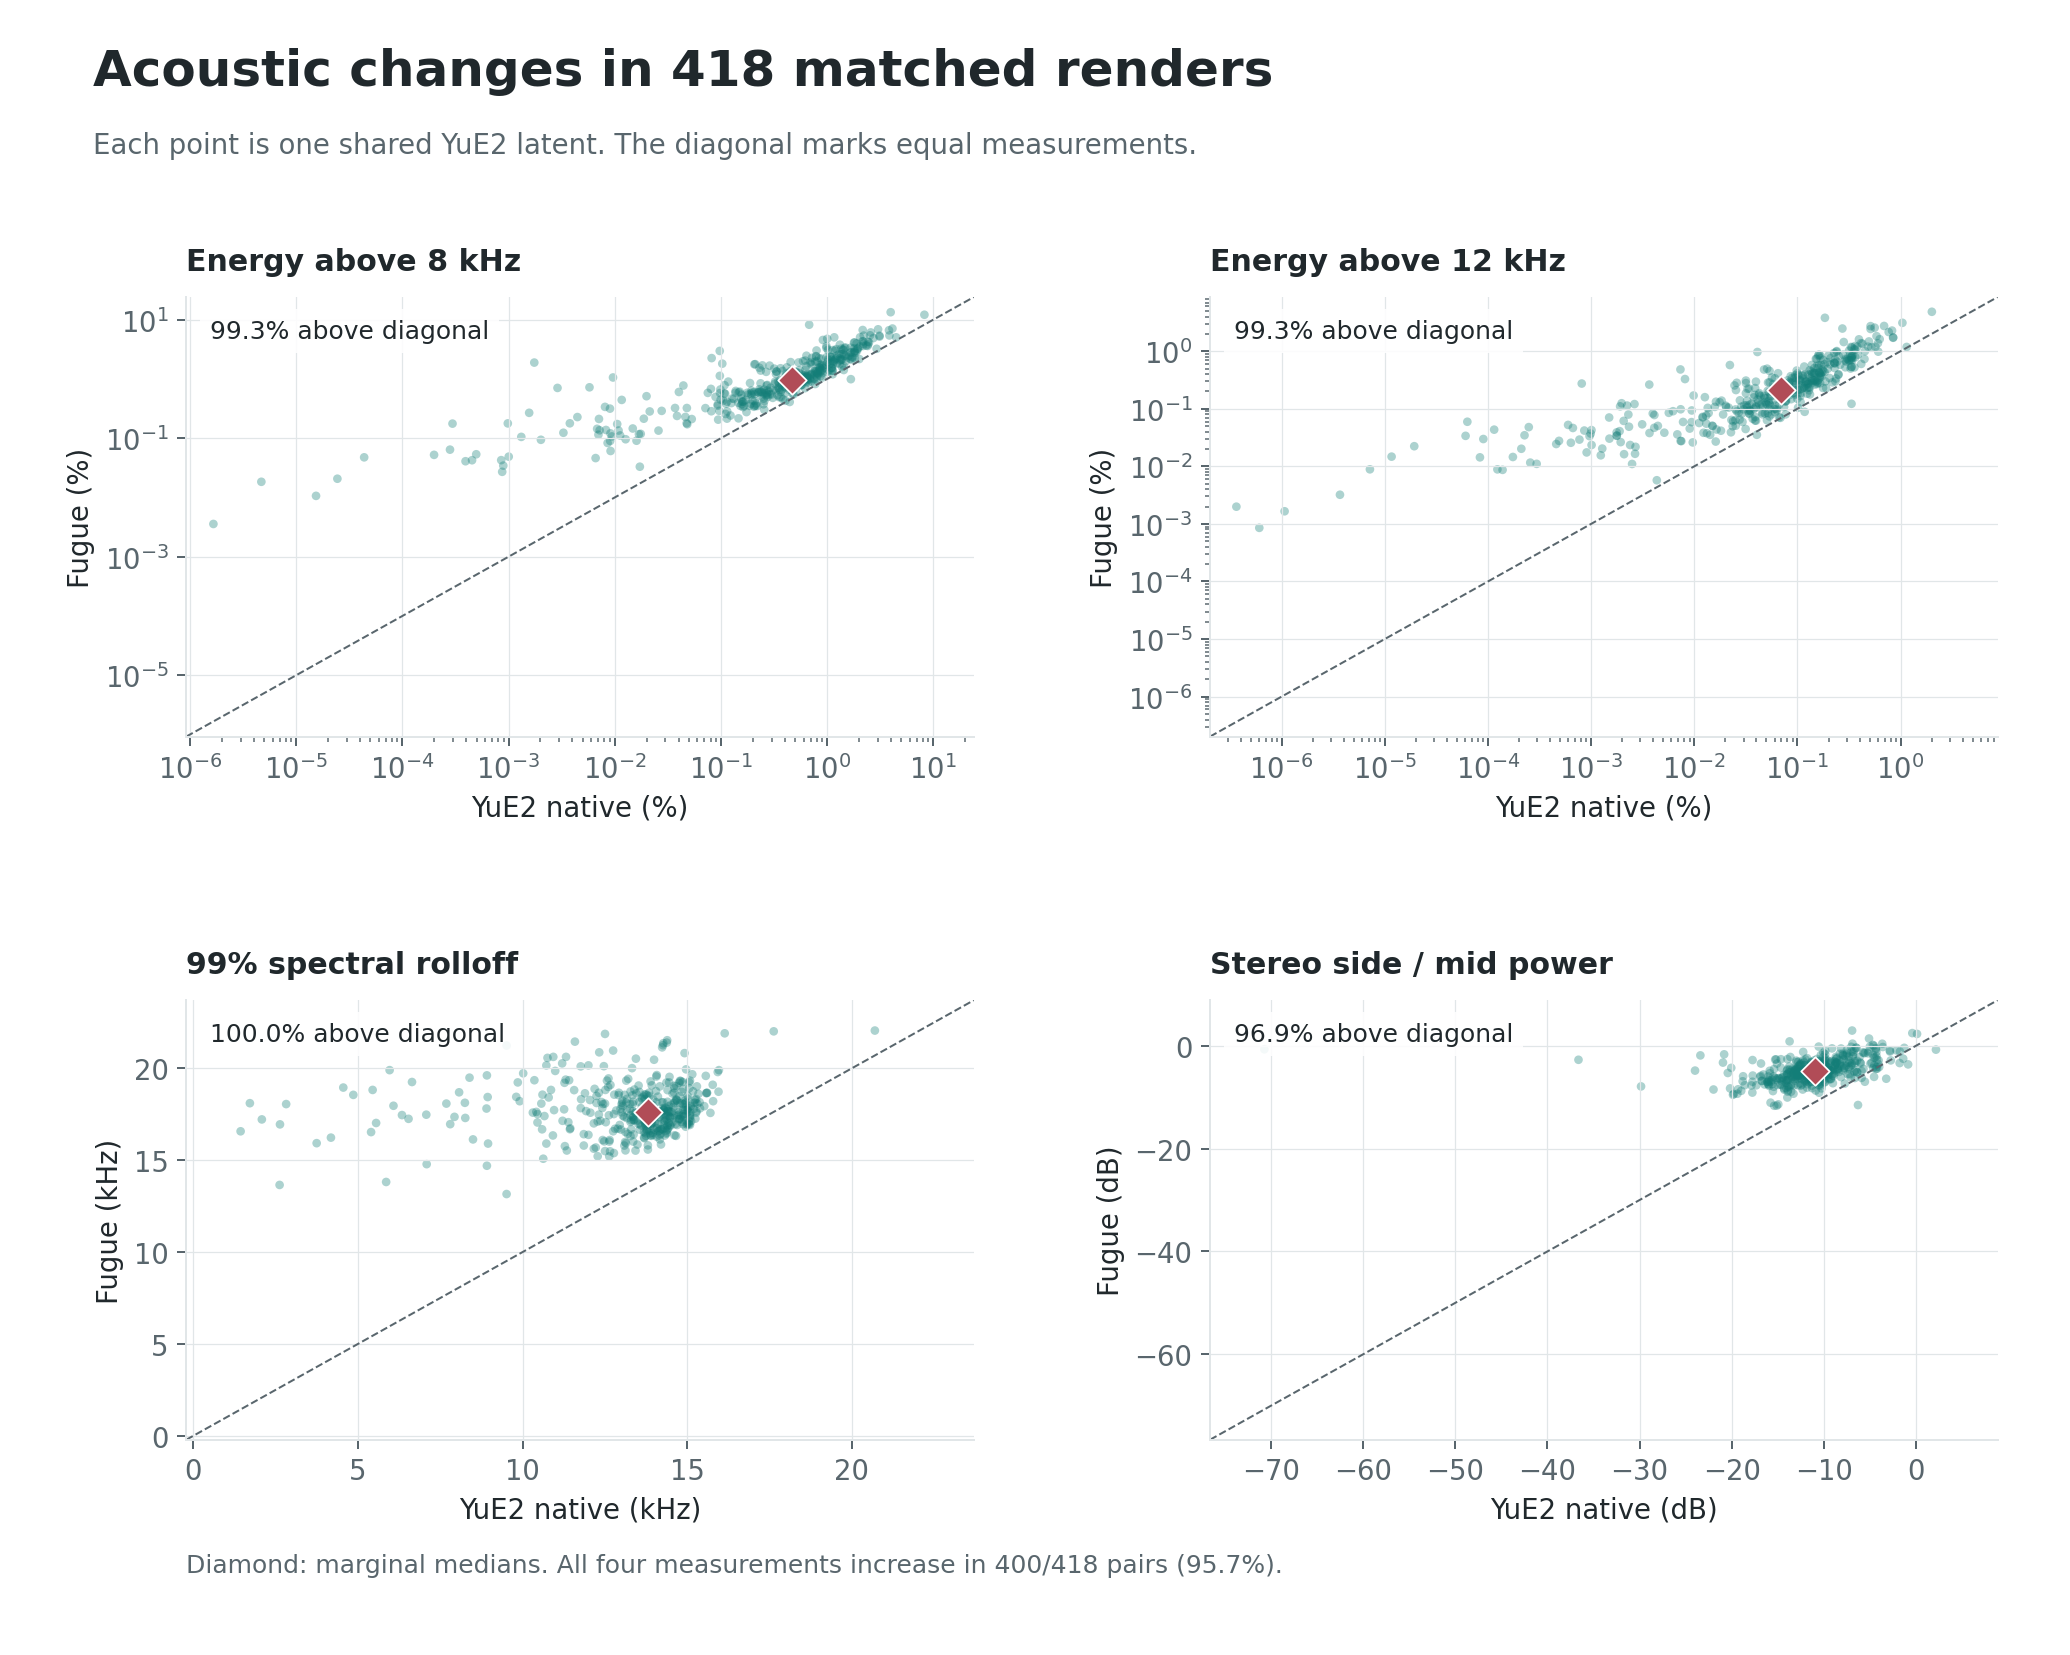
\includegraphics[width=0.96\linewidth]{acoustic-changes.png}
    \caption{418 对配对渲染结果的声学变化。高频段能量采用对数坐标轴；滚降频率与立体声功率采用线性坐标轴。菱形标记的位置由两个坐标变量各自的中位数确定。位于对角线上方表示所绘测量值增加，并不代表感知偏好投票。}
    \label{fig:acoustic}
\end{figure}

\begin{table}[htbp]
    \centering
    \caption{频谱与立体声测量。四项指标在 400/418 对输出（95.7\%）中同时增加。}
    \label{tab:acoustic}
    \small
    \begin{tabular}{lrrr}
        \toprule
        测量项 & YuE2 原生解码器中位数 & Fugue 中位数 & 数值增加的配对数 \\
        \midrule
        8 kHz 以上能量 & 0.466\% & 0.966\% & 415/418 (99.3\%) \\
        12 kHz 以上能量 & 0.070\% & 0.209\% & 415/418 (99.3\%) \\
        99\% 频谱滚降频率 & 13.8 kHz & 17.6 kHz & 418/418 (100\%) \\
        立体声侧声道/中声道功率比 & $-10.9$ dB & $-4.8$ dB & 405/418 (96.9\%) \\
        \bottomrule
    \end{tabular}
\end{table}

配对差值的中位数，滚降频率为 $+3.8$ kHz，侧声道/中声道功率比为 $+6.1$ dB。高频段能量由单声道功率谱测量。滚降频率的计算方式是：逐帧求出累积幅度谱达到 99\% 时的频率，再取中位数。立体声宽度以 $10\log_{10}\bigl(\operatorname{var}(L-R)/\operatorname{var}(L+R)\bigr)$ 报告，使用 \code{eval\_score.py} 中的数值稳定项。

当前版本中，Audiobox-Aesthetics PQ 的配对下降量中位数为 0.278。我们将其与频谱和立体声测量一并报告：更多高频成分和更大的立体声宽度，本身并不构成更高感知音质的主张。在另一项基于真实录音的编解码往返案例研究中，YuE2 VAE 的 SI-SDR 为 7.7 dB，MM3 Flow-VAE 为 17.7 dB。该实验衡量的是编解码器的重建能力，与生成全新编曲是不同的问题。

\subsection{基准集之外的全长改编}
\label{sec:showcase}

\begin{figure}[t]
    \centering
    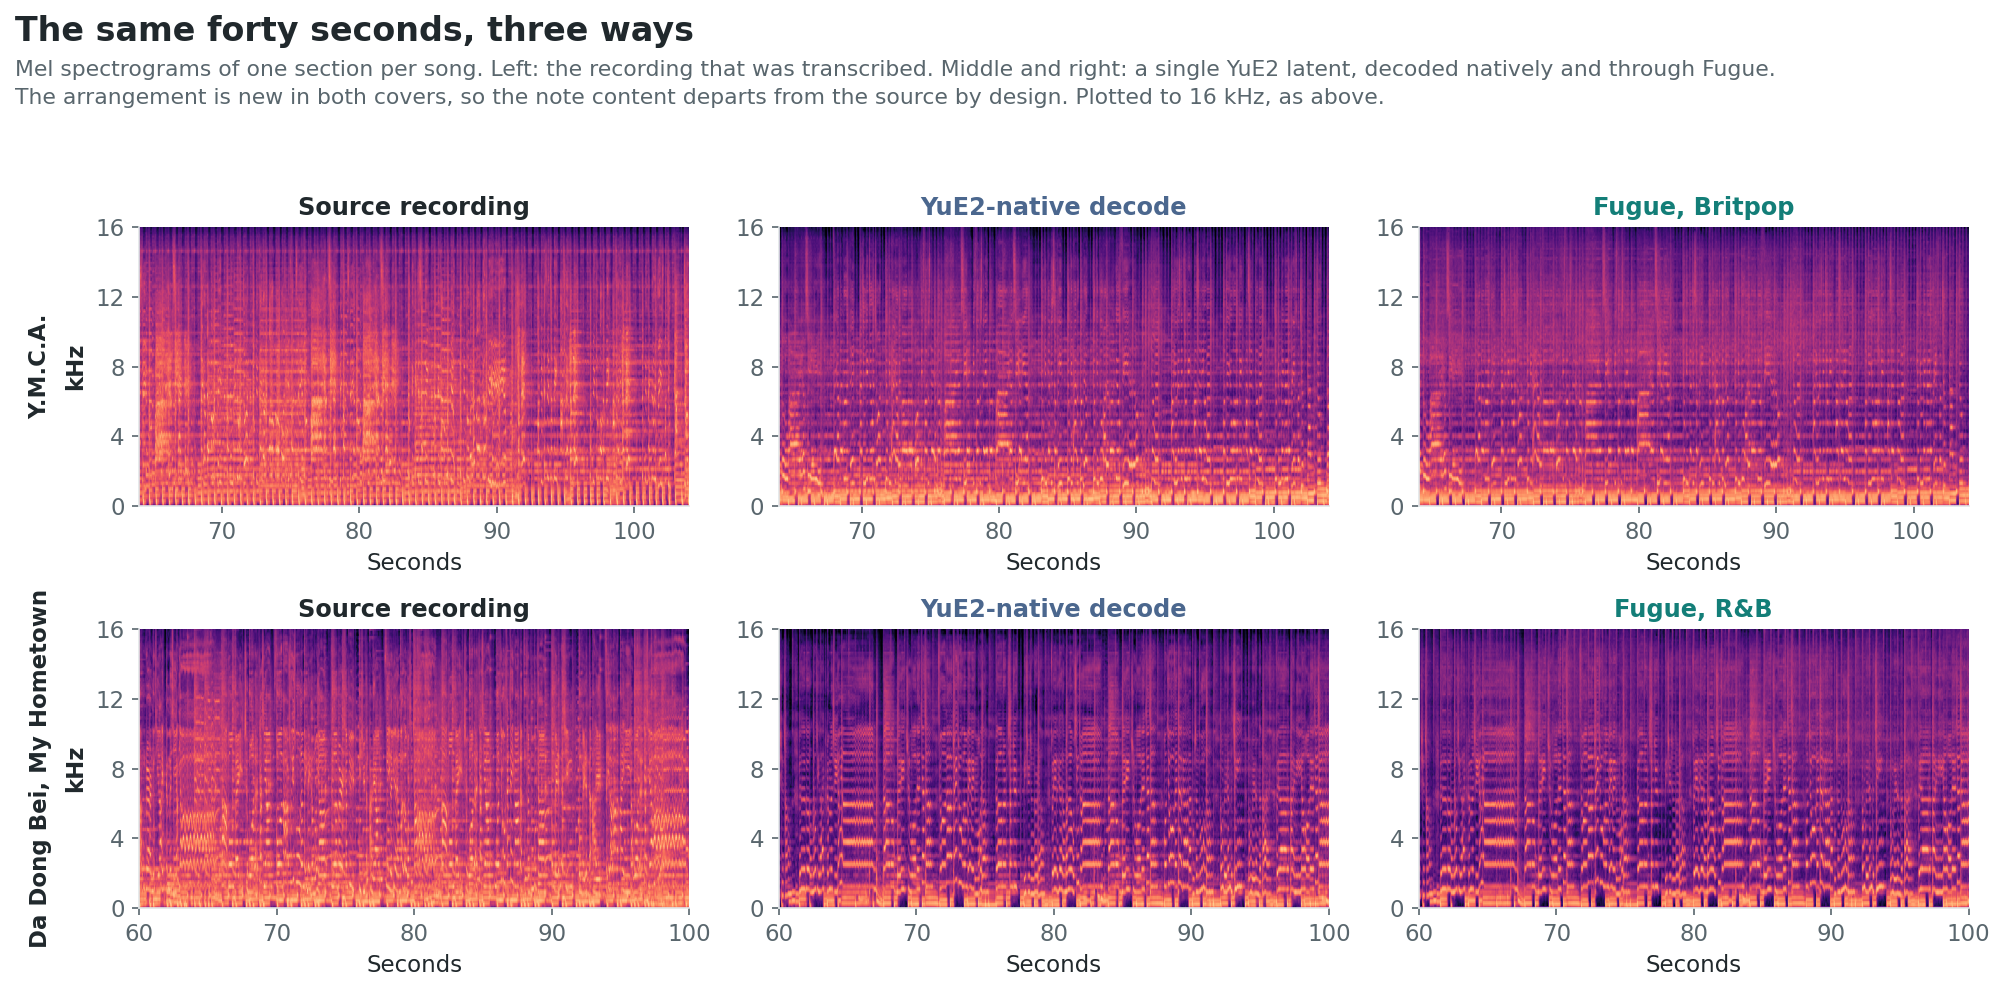
\includegraphics[width=\linewidth]{real-song-covers.png}
    \caption{两首歌曲同样的四十秒，三种呈现方式。行对应两首源录音；列依次为原曲、所生成潜表示的 YuE2 原生解码，以及同一潜表示的 Fugue 渲染。梅尔谱绘制至 16 kHz，这样无损原曲与 MP3 试听在 8 kHz 以上仍可比较，而不会把 MP3 编码器自身的低通特性带入对比。}
    \label{fig:showcase-mel}
\end{figure}

\begin{figure}[t]
    \centering
    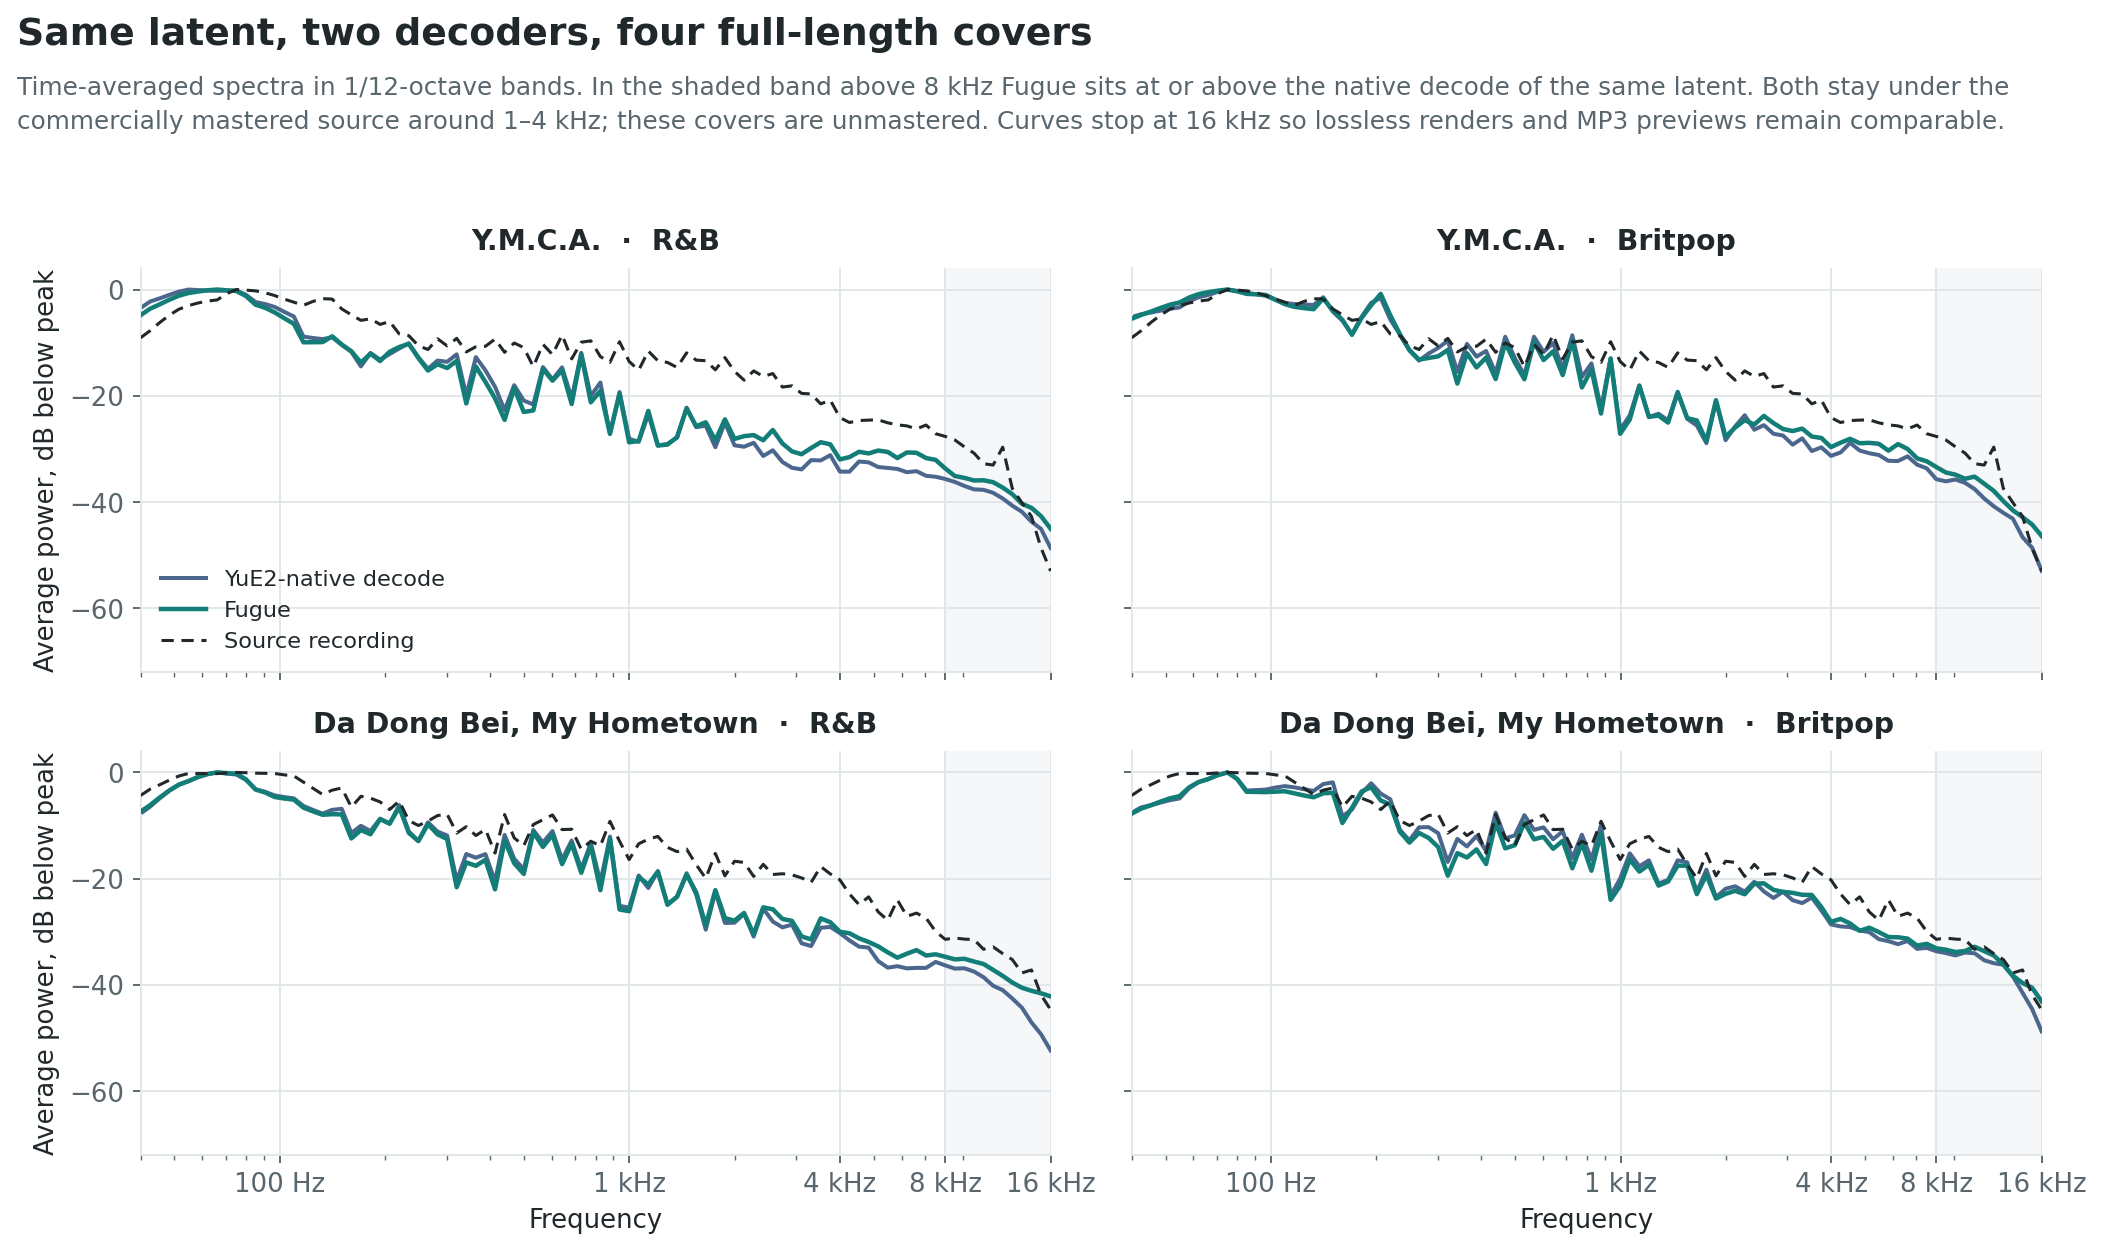
\includegraphics[width=\linewidth]{real-song-spectra.png}
    \caption{四首全长改编的时间平均频谱，按 1/12 倍频程分带汇总并绘制至 16 kHz。行为歌曲，列为目标风格；每格叠加原曲录音、YuE2 原生解码，以及同一潜表示的 Fugue 渲染。阴影区标出 8--16 kHz。在这几首曲目上，Fugue 处于同一潜表示原生解码的水平或之上；差距是几 dB，而非数量级。}
    \label{fig:showcase-spectra}
\end{figure}

上述基准生成结果均为纯器乐、时长 60 秒。作为另一组展示，我们对基准曲库之外的两首真实录音各生成两种风格、带人声的全长改编。SheetSage2 将每首原曲转录为带和弦标注的双声部 ABC 乐谱，歌词以文本形式提供，而非由 ASR 识别得到。同一首歌的两个改编版本复用同一份乐谱和同一份歌词，因此风格提示词与 YuE2 随机种子是仅有的变量；提示词中不含 BPM，速度由 ABC 自带的速度行决定。每条音轨均为一次生成、无拼接，时长 243--284 秒，在单张 RTX 4090 上的墙钟时间为 171--204 秒。图~\ref{fig:showcase-mel}~和图~\ref{fig:showcase-spectra}~将这些音轨与其原曲、以及同一潜表示的原生解码放在一起对比。

这四条音轨是定性展示，且是从更大的一批生成结果中凭耳朵挑选出来的，因此不应被视为表~\ref{tab:acoustic}~中声学趋势的无偏样本。逐条与各自原曲相比，它们的走向并不一致：Y.M.C.A.\ 的英伦摇滚版 8 kHz 以上能量占 0.89\%、滚降频率为 7.6 kHz，低于其原曲录音，而另外三条则高于各自原曲。单曲层面的渲染结果取决于生成器实际产出的内容，而非一条会单调抬升高频的渲染路径。此外，原曲是商用母带，而改编没有任何母带处理环节，曲线之间可见的电平差异大多源于此。

% ══════════════════════════════════════════════════════════════
\section{接口分析}
% ══════════════════════════════════════════════════════════════

\subsection{学到了什么}

\begin{table}[htbp]
    \centering
    \caption{开发阶段各次实验的条件预测结果。岭回归与神经适配器实验使用不同的拟合/评估子集，因此本表并非受控的规模扩展对比。v4 验证使用 150 首留出歌曲。$R^2$ 以训练集各通道的均值为基准；它衡量的是条件回归效果，而非改编质量。}
    \label{tab:learned}
    \small
    \begin{tabular}{lrr}
        \toprule
        适配器或探针 & 方差加权 $R^2$ & 通道平均 $R^2$ \\
        \midrule
        岭回归，使用 17 帧上下文的 YuE2 潜表示 & 0.384 & 0.150 \\
        岭回归，使用 17 帧上下文的池化 MM3 DAV 潜表示 & 0.201 & 0.086 \\
        v1：6 层，宽度 512，1,050 首训练歌曲 & 0.593 & 0.369 \\
        v2：8 层，宽度 768，10,340 首训练歌曲 & 0.665 & 0.464 \\
        v3：在 v2 基础上使用方差加权损失 & 0.672 & 0.462 \\
        \textbf{v4：在 v3 基础上加入输入噪声，发布版本} & \textbf{0.671} & \textbf{0.461} \\
        \bottomrule
    \end{tabular}
\end{table}

在所测试的线性读出方式下，YuE2 潜表示比池化后的 MM3 DAV 潜表示具有更强的预测能力。Transformer 适配器对条件的拟合优于岭回归基线。

输入噪声增强几乎不改变验证集 $R^2$。在真实歌曲的钢琴改编案例研究中，v4 将重新转录后的 DTW 从 v3 的 0.434 降至 0.369，作为对照，YuE2 原生解码器为 0.353。在一个 MM3 重建案例中，v4 将 log-mel L1 从 v3 的 0.787 降至 0.740。这些案例促成了发布版本的选择；209 首歌曲的基准评估针对 v4，而非对所有版本进行消融实验。

\subsection{渲染器敏感性}

\begin{table}[htbp]
    \centering
    \caption{对一个 MM3 生成的英伦摇滚示例进行的条件扰动实验。每一行均将输出与已保存的原始音频进行比较。另行测得的不同随机种子渲染结果之间的距离为 0.698。}
    \label{tab:sensitivity}
    \small
    \begin{tabular}{lr}
        \toprule
        30 秒重建案例中使用的条件 & 与已保存原始音频的 log-mel L1 距离 \\
        \midrule
        教师强制恢复的条件，DiT 随机种子 7 / 随机种子 8 & 0.686 / 0.703 \\
        添加噪声，噪声方差为各通道方差的 10\% / 30\% & 0.697 / 0.729 \\
        Fugue v4 根据编码后的音频预测的条件 & 0.740 \\
        全零条件 & 2.279 \\
        另一首歌的条件 & 5.077 \\
        \bottomrule
    \end{tabular}
\end{table}

该案例表明，渲染器能够容忍中等程度的非结构化条件误差，同时仍对移除或替换条件保持敏感。学习得到的适配器残差具有结构性，其行为可能与高斯噪声不同。

原生条件投影和帧率见附录~\ref{app:native}。

\subsection{基础设施贡献}
\label{sec:infra}

\paragraph{训练与发布流水线。}Fugue 提供了从已保存生成编码恢复 MM3 条件、用 YuE2 编码对应音频、对齐两端时间轴、计算通道统计量及训练适配器的工具。推理包将适配器权重、归一化统计量和分块配置作为一组配套发布产物加载。这一封装使学习得到的接口能够在改编生成路径中运行，而无需 MM3 的语言模型或深度解码器。研究脚本保留了实验环境特定的路径；推理包则提供可配置的模型位置。

\paragraph{常驻服务与编排。}\href{https://github.com/HenryZ838978/fugue/tree/main/services}{服务实现}将转录/YuE2 生成与适配器/MM3 渲染分离，使两套依赖环境保持独立，同时允许模型共享一张 GPU。各阶段通过 HTTP 请求协调，以共享文件系统上的潜表示文件传递中间表示。模型在多次请求之间保持常驻，转录服务在完成转录后释放未使用的 CUDA 缓存，为渲染服务留出显存。服务流程记录请求、中间潜表示、各阶段耗时和输出，并为生成与渲染分别设置随机种子。

\paragraph{长音频推理与用户接口。}\href{https://github.com/HenryZ838978/fugue/tree/main/fugue}{推理包}实现了带两侧上下文的适配器窗口，并将输出接入 MM3 原生的分块去噪与波形拼接流程。这里的贡献是让学习得到的接口与既有渲染调度协同工作，而非提出新的 DiT 或声码器。单进程 CLI 接受录音或 ABC 乐谱、目标风格及可选歌词；基于服务的 CLI 和 Arena 前端提供相同的改编流程。已发布的 Arena 展示带标签的原曲、YuE2 原生解码和 Fugue 输出，用于对比，而非实施盲听研究。

\paragraph{配对评估与可审查性。}\href{https://github.com/HenryZ838978/fugue/blob/main/research/eval_gen.py}{基准运行脚本}支持生成任务分片、重跑时跳过已完成条目，并将每个生成潜表示送入两个解码器。逐输出记录保存原曲/风格分配及生成元数据。已发布的评分与绘图工具将这些记录关联到汇总表格和配对计数。这套基础设施支持结果检查及后续评估扩展，同时避免将不同上游生成结果的差异与渲染器变化混为一谈。

\subsection{运行时间与长篇示例}

在作为参考的 24 GB GPU 上，常驻的转录/YuE2 服务和嫁接/渲染服务分别占用约 9.8 GB 和 4.9 GB 显存。一段 30 秒改编的端到端耗时约为 50 秒。一个时长为 4:37 的钢琴输出，其 AR、NAR 和声学渲染耗时分别为 54、23 和 118 秒。这些单次运行均使用常驻模型；长篇示例实际运行了分块推理路径。

% ══════════════════════════════════════════════════════════════
\section{讨论：一种实用的替代方案}
% ══════════════════════════════════════════════════════════════

预训练生成器的默认推理流程未必就是它最终的接口。Fugue 是\textbf{预训练后外部适配}的一个实例：学习得到的桥接模块改变了哪些上游音乐表示可以驱动渲染器，而原始权重始终保持固定。新增的音乐改编能力属于组合后的系统，而非一个新近接受了乐谱训练的 MM3 主干模型。

系统定位为\textbf{乐谱条件音乐改编的一种实用替代方案，提供更多高频成分与更宽立体声声场}。YuE2 提供乐谱条件音乐生成，MM3 提供预训练的 DiT 渲染能力。Fugue 的贡献是学习得到的连接方式、来自自生成数据的监督，以及运行和评估组合系统的基础设施。这一区分既体现了完整改编流程的价值，也避免将上游原有能力归为 Fugue 的新贡献。

工程上的问题是：如何连接这些能力，同时让渲染器保持在有效的条件输入范围内。在本研究中，这一问题引导我们采用原生条件目标、时间对齐、通道归一化和输入增强。当前版本的检索差距表明，接口层面仍有需要研究的局限，而非证明冻结模型组合必然付出这一代价。本文评估的是这一版本，并未建立相对于其他改编系统的总体排名。

% ══════════════════════════════════════════════════════════════
\section{相关工作}
% ══════════════════════════════════════════════════════════════

\paragraph{乐谱条件音乐生成。}YuE2~\cite{yue2} 提供 Fugue 所使用的读谱与生成能力。MM3~\cite{mm3} 提供声学渲染器。本文的贡献在于二者的组合及其训练方案，并通过本地配对解码器研究单独考察这一组合的效果。

\paragraph{冻结模型组合。}Foley Control~\cite{foleycontrol} 通过新增交叉注意力，将冻结的视频嵌入连接到冻结的文本到音频 DiT，以视频作为声音生成的条件。相比之下，Fugue 根据另一个音乐生成器的声学潜表示，预测渲染器现有的条件表示，监督信号则从渲染器自身的生成结果中恢复。Freeze-Omni~\cite{freezeomni} 同样表明，可以利用语音/文本监督，在冻结的语言模型周围学习语音接口。Fugue 的桥接模块无需额外提供目标任务中从原曲到改编曲的转换示例。

\paragraph{表示与读出。}\emph{Where Does the Sound Go?}~\cite{soundgo} 发现，即使下游回答未能利用声学信息，这些信息仍可能从音频条件 LLM 的表示中恢复出来，提示问题可能在于读出对齐。这促使我们区分表示中可用的信息与接收端实际表现出的行为。Fugue 检验的是冻结模块之间学习得到的接口；本文报告的结果针对这一接口，而非直接操纵激活。

% ══════════════════════════════════════════════════════════════
\section{当前版本的局限性与发布后 V2 计划}
% ══════════════════════════════════════════════════════════════

当前 Fugue v4 基准使用包含 210 段录音的检索库、单一 YuE2 随机种子、60 秒纯器乐生成结果，以及范围有限的原曲曲库。人声可懂度、听众偏好、长篇一致性和对更广泛曲风的泛化能力，仍需专门评估。适配器拟合的是 MM3 生成音频的编码，而推理时使用的是 YuE2 生成的潜表示。部分开发示例表现出与渲染器有关的音色偏移。检索与 PQ 结果刻画了当前版本的局限，与其更多高频成分和更宽立体声声场一并呈现。

当前接口通过所提供的乐谱和风格提示词控制完整的混合音频生成。它不保证指定分轨保持不变、精确复制音符，或独立编辑人声与器乐旋律线。

首次发布先开放系统及其当前评估结果，计划在发布后的\textbf{本报告 V2 修订版}中补充以下研究；这里的报告修订版不应与表~\ref{tab:learned}~中早期的 v2 适配器实验混淆：

\begin{enumerate}[leftmargin=2em,itemsep=0.25em]
    \item \textbf{Arena 盲听：}由独立听众参与随机、响度匹配的对比，分别评估音质、原曲辨识度、目标风格符合度和总体偏好。
    \item \textbf{音乐改编基线：}在匹配的原曲、目标风格和生成预算下，与其他改编系统比较，扩展检索库，并明确报告失败输出。
    \item \textbf{受控子集消融：}在同一个留出改编子集上测试时间对齐、输入噪声和损失加权，使用多个随机种子考察当前的检索差距与渲染变化。
\end{enumerate}

以上均为发布后计划补充的工作，不是当前版本已经完成或宣称的实验结果。

% ══════════════════════════════════════════════════════════════
\appendix
\section{在 MM3 上直接引入乐谱条件的尝试}
\label{app:direct}
% ══════════════════════════════════════════════════════════════

在构建嫁接方案之前，我们曾在 MM3 上尝试文本前缀、token 前缀和流内条件注入路径。教师强制诊断指标为 $d_{\mathrm{spec}} = \mathrm{CE}(\text{other-score}) - \mathrm{CE}(\text{true-score})$：正值越大，说明真实乐谱越有助于预测音频编码。

\begin{table}[H]
    \centering
    \caption{在 MM3 上直接引入乐谱条件的尝试，YuE2 对照使用同一诊断指标测得。}
    \label{tab:direct}
    \footnotesize
    \begin{tabular}{llrr}
        \toprule
        实验 & 条件注入路径 & $d_{\mathrm{spec}}$ & 差值为正的配对数 \\
        \midrule
        r1 / r2 & ABC 文本前缀 & 约为 0 & 未列出 \\
        Stage A & 编解码器 token 前缀 & 约为 0 & 未列出 \\
        r3 & 流内与前缀 & $+0.0003$ & 26/48 \\
        r4 & 计划损失、条件丢弃、保留速度信息 & $+0.0025$ & 18/24 \\
        YuE2 对照 & ABC 文本前缀 & $+0.340$ & 24/24 \\
        \bottomrule
    \end{tabular}
\end{table}

在 r4 中，ABC 生成损失从 23.1 降至 0.49，但基于乐谱条件的音频预测未出现相应幅度的改善。在所测试的设置下，学会生成 ABC 并未转化为对音频预测有效的乐谱条件控制能力。这些实验促使我们转而复用 YuE2 的既有能力。

% ══════════════════════════════════════════════════════════════
\section{原生条件与可复现性}
\label{app:native}
% ══════════════════════════════════════════════════════════════

MM3 的 \code{ConditionEncoder} 将语言模型隐藏状态和七个 RVQ 深度隐藏状态进行 softmax 加权求和，乘以一个可学习的标量，再用卷积核大小为 3 的卷积从 4096 通道投影至 2048 通道。实测混合系数约为 $[0.906, 0.013, 0.013, 0.013, 0.014, 0.014, 0.014, 0.014]$，标量为 0.0685。由于模型其他位置还存在投影和归一化，不能仅将该标量解释为条件作用的强度。

条件帧率为 $24000/960 = 25$ Hz；声学潜表示帧率为 $44100/512 = 86.1328125$ Hz。标称上采样比为 $441/128 = 3.4453125$，每个分块的输出长度取整数。这些数值是表示的帧率，并非波形频率内容的上限。

已发布的\href{https://github.com/HenryZ838978/fugue/blob/main/research/eval_summary.json}{汇总结果}和\href{https://github.com/HenryZ838978/fugue/blob/main/research/eval_per_item.json}{逐输出记录}为表~\ref{tab:identity}--\ref{tab:acoustic}~和图~\ref{fig:identity}--\ref{fig:acoustic}~提供数据支持。\href{https://github.com/HenryZ838978/fugue/blob/main/paper/figures/render_figures.py}{绘图脚本}根据逐输出记录验证汇总结果，计算配对计数，并导出 SVG 和 PNG；\href{https://github.com/HenryZ838978/fugue/blob/main/paper/figures/render_showcase.py}{另一个脚本}依据展示音频及其已存曲线绘制图~\ref{fig:showcase-mel}~和图~\ref{fig:showcase-spectra}。表~\ref{tab:learned}--\ref{tab:sensitivity}~的开发阶段分析记录在\href{https://github.com/HenryZ838978/fugue/blob/main/research/SCION.md}{历史实验笔记}中。\href{https://github.com/HenryZ838978/fugue/blob/main/samples/README.md}{样例索引}列出了试听音频及其生成设置。

% ══════════════════════════════════════════════════════════════
\begin{thebibliography}{9}
\small\raggedright\setlength{\itemsep}{2pt}
\bibitem{yue2} M-A-P. \emph{YuE2-3B}. 模型卡与推理实现，2026。Hugging Face 模型标识：\code{m-a-p/YuE2-3B}。

\bibitem{mm3} MiniMax. \emph{MiniMax-Music3}. 模型发布，2026。Hugging Face 模型标识：\code{MiniMaxAI/MiniMax-Music3}。

\bibitem{discogsvi} R. Oguz Araz, Xavier Serra, and Dmitry Bogdanov. \emph{Discogs-VI: A Musical Version Identification Dataset Based on Public Editorial Metadata}. ISMIR, 2024. arXiv:2410.17400.

\bibitem{foleycontrol} Ciara Rowles et al. \emph{Foley Control: Aligning a Frozen Latent Text-to-Audio Model to Video}. 2025. arXiv:2510.21581.

\bibitem{freezeomni} Xiong Wang et al. \emph{Freeze-Omni: A Smart and Low Latency Speech-to-speech Dialogue Model with Frozen LLM}. 2024. arXiv:2411.00774.

\bibitem{soundgo} Song-ha Jo et al. \emph{Where Does the Sound Go? Tracing Acoustic Information Loss in Audio-Conditioned LLMs}. 2026. arXiv:2609.05871.
\end{thebibliography}

\end{document}
